\chapter{Background}

In this chapter, I am going to introduce the concepts that are necessary to understand the research presented in this thesis. The chapter is divided into five sections. The first section provides an overview of Variational Autoencoders (VAEs) and their applications. The second section introduces Vector Quantized VAEs (VQ-VAEs). The third section introduces the concept of semi-conditioned VAEs. The fourth section introduces the concept of multitask learning. The chapter concludes with a section that delves into additional concepts that are necessary to understand the research presented in this thesis.

\section{VAEs}

Variational Autoencoders (VAEs), first introduced in 2013 by Kingma and Welling~\cite{kingma2013autoencoding}, have become a prominent class of generative models in the field of machine learning.  At their core, VAEs consist of an encoder network with parameters $\phi$ that maps data points $x$ into a latent space $z$ and a decoder network with parameters $\theta$ that generates data $\hat{x}$ from latent representations~\cite{Kingma_2019}. 

The key innovation that makes VAEs work is the introduction of a probabilistic interpretation of the latent space. More specifically, VAEs assume that the latent space $z$ is a random variable that follows a certain prior distribution $p(z)$, which is typically a Gaussian distribution and that the mapping from the latent space to the data space is also probabilistic~\cite{kingma2013autoencoding}.

The optimization target for VAEs is the evidence lower bound (ELBO), which is
 \[ L_{\theta, \phi}(x) = \mathbb{E}_{q_{\phi}(z|x)} [\log p_{\theta}(x, z) - \log q_{\phi}(z|x)], \]
where $q_{\phi}(z|x)$ is the encoder distribution, $p_{\theta}(x, z)$ is the decoder distribution. 

The ELBO can be also written as a sum of two terms,
 \[ L_{\theta, \phi}(x) = - D_{KL}(q_{\phi}(z|x) || p(z)) + \mathbb{E}_{q_{\phi}(z|x)} [\log p_{\theta}(x|z)], \]
 where:

\begin{itemize}
    \item $D_{KL}(q_{\phi}(z|x) || p(z))$ is the Kullback-Leibler divergence between the encoder distribution $q_{\phi}(z|x)$ and the prior distribution $p(z)$
    \item $\mathbb{E}_{q_{\phi}(z|x)} [\log p_{\theta}(x|z)]$ is the reconstruction term
\end{itemize}

The Kullback-Leibler divergence term encourages the encoder (posterior) distribution to align with the prior distribution, acting as a regularization term. This alignment is crucial for an effective utilization of the latent space. On the other hand, the reconstruction term encourages the decoder to reconstruct the input data as accurately as possible, which encourages the decoder to accurately capture the data distribution.

While the expression of the ELBO might appear different from the original formulation, it remains equivalent, merely using different terms to express the same notion~\cite{Kingma_2019}.

Sampling from $q_{\phi}(z|x)$ involves drawing samples denoted as $z^{(l)} \sim q_{\phi}(z|x)$, enabling the Monte Carlo estimation—a method for numerical approximation using random sampling—of the following objective function:
\[ L_{\theta, \phi}(x) = - D_{KL}(q_{\phi}(z|x) || p(z)) + \frac{1}{L} \sum_{l=1}^{L} \log p_{\theta}(x|z^{(l)}) ,\]
where $L$ represents the number of samples drawn, as described in~\cite{Kingma_2019}.


The individual data point ELBO and its gradients are in general intractable to compute. However, unbiased estimates of the ELBO and its gradients can be obtained using the reparameterization trick, which is described in the next section~\cite{Kingma_2019}.

\subsection{The reparameterization trick}

The reparameterization trick also is a crucial component of VAEs. It is used to make the ELBO differentiable with respect to the parameters of the encoder $\phi$ and decoder $\theta$ through a change of variables~\cite{Kingma_2019}.

\subsubsection{Change of variables}

The notion is based on the fact that it is possible to express the random variable $z \sim q_{\phi}(z|x)$ as a differentiable function of a random variable $\epsilon$ and the parameters $\phi$ such that $z = g_{\phi}(\epsilon, x)$, where $\epsilon$ is a random variable that is independent of $\phi$ and $x$ and $\epsilon \sim p(\epsilon)$. Given this change of variables, the expectation with respect to $q_{\phi}(z|x)$ can be rewritten as an expectation with respect to $p(\epsilon)$
\[ E_{q_{\phi}(z|x)}[f(z)] = E_{p(\epsilon)}[f(g_{\phi}(\epsilon, x))], \]
where $f$ is an arbitrary function~\cite{Kingma_2019}.
As a result, the gradients of the expectation and gradient operators become commutative, and there can be formed a Monte Carlo estimate of the gradients
\[ \nabla_{\phi} E_{q_{\phi}(z|x)}[f(z)] = \nabla_{\phi} E_{p(\epsilon)}[ f(g_{\phi}(\epsilon, x))] \]
\[ = E_{p(\epsilon)}[\nabla_{\phi} f(g_{\phi}(\epsilon, x))] \]
\[  \simeq \frac{1}{L} \sum_{l=1}^{L} \nabla_{\phi} f(g_{\phi}(\epsilon^{(l)}, x)) \]
where $\epsilon^{(l)} \sim p(\epsilon)$ and $L$ is the number of samples~\cite{Kingma_2019}.
This is the reparameterization trick, which is further explained and illustrated in the figure~\ref{reparametrization}.

\begin{figure}
    \centering
    \begin{tikzpicture}[
    roundnode/.style={circle, draw=red!60, fill=red!5, very thick, minimum size=7mm},
    squarednode/.style={rectangle, draw=gray!60, fill=gray!5, very thick, minimum size=5mm},
    redarrow/.style={->, red, >=stealth, thick},
    redtext/.style={red}
    ]

    % Two boxes with widht of full text
    \draw (0,0) rectangle (6, 6);
    \draw (7,0) rectangle (13, 6);
    % Headlines
    \node[align=center] at (3,5.5) {Original Form};
    \node[align=center] at (10,5.5) {Reparametrized Form};

    % --- First box ---
    %Nodes
    \node[squarednode]      (function)      at(3, 4.5)                    {$f$};
    \node[roundnode]        (z)             [below= of function]          {$z$};
    \node[squarednode]      (x)             [below= of z]                 {$x$};
    \node[squarednode]      (phi)         [left= of x]        {$\phi$};
    %Lines
    \draw [->] (z) -- (function);
    \draw [->] (x) -- (z);
    \draw [->] (phi) -- (z);

    % --- Second box ---
    %Nodes
    \node[squarednode]      (function2)      at(10, 4.5)                    {$f$};
    \node[squarednode]        (z2)             [below= of function2]          {$z$};
    \node[squarednode]      (x2)             [below= of z2]                 {$x$};
    \node[squarednode]      (phi2)         [left= of x2]        {$\phi$};
    \node[roundnode]        (epsilon)        [right= of x2]        {$\epsilon$};
    %Lines
    \draw [->] (z2) -- (function2);
    \draw [->] (x2) -- (z2);
    \draw [->] (phi2) -- (z2);
    \draw [->] (epsilon) -- (z2);

    % draw back propagation with red line draw to the left
    \draw [redarrow] (9.5, 4.5) -- (9.5, 3.3);
    \node [redtext, above left= -0.3 and 0.3 of z2] { $\nabla_{z} f$};
    \draw [redarrow] (9.5, 3) -- (8.5, 2);
    \node [redtext, above left= -0.1 and -0.1 of phi2] { $\nabla_{\phi} f$};
    % One box below to show the meaning of nodes and lines
    \draw (0,-3) rectangle (13, -0.5);
    %show the meaning of nodes 
    \node[squarednode]    (square_explanation_node)    at(1, -1)    {};
    \node [right= 0.5 of square_explanation_node] {: Deterministic node};
    \node[roundnode]    (round_explanation_node)    at(1, -2)    {};
    \node [right= 0.5 of round_explanation_node] {: Random node} ;
    %\draw (5.5, -2)    node    {: Random node};
    %show the meaning of lines( with name of the line)
    \draw [->] (7, -1) -- (8, -1) node [right = 0.5,] { : Calculation of f};
    \draw [redarrow] (7, -2) -- (8, -2) node [right = 0.5,] { : Differentiation of f};
\end{tikzpicture}
    \caption[Illustration diagram of the reparameterization trick]%
    {Illustration diagram of the reparameterization trick. The input of a function $f$ is $x$. The parameters $\theta$ affect the objective of the function $f$ through a random variable $z$. In the original form, we can not compute the gradients $\nabla_{\phi} f$, because direct backpropagation is not possible through a random variable. In the reparameterized form, the randomness is separated from the parameters $\phi$, which enables the gradients to be computed. This is done by reparameterizing the random variable $z$ as a deterministic function and differentiable function of $\phi$, $x$ and a new random variable $\epsilon$~\cite{Kingma_2019}}.

    \hspace*{15pt}\hbox{\scriptsize Credit: Adapted from Kingma and Welling\cite{Kingma_2019}  }\label{reparametrization}

\end{figure}

\subsubsection{Gradients of the ELBO}

When applying the reparameterization trick to the ELBO it becomes differentiable with respect to both $\phi$ and $\theta$, and it is possible to form a Monte Carlo estimate of the gradients
\[ \nabla_{\phi, \theta} L_{\theta, \phi}(x) = \nabla_{\phi, \theta} E_{q_{\phi}(z|x)} [\log p_{\theta}(x, z) - \log q_{\phi}(z|x)] \]
\[ = E_{p(\epsilon)}[\nabla_{\phi, \theta} [\log p_{\theta}(x, g_{\phi}(\epsilon, x)) - \log q_{\phi}(g_{\phi}(\epsilon, x)|x)]] \]
\[  \simeq \frac{1}{L} \sum_{l=1}^{L} \nabla_{\phi, \theta} [\log p_{\theta}(x, g_{\phi}(\epsilon^{(l)}, x)) - \log q_{\phi}(g_{\phi}(\epsilon^{(l)}, x)|x)] \]
where $\epsilon^{(l)} \sim p(\epsilon)$ and $L$ is the number of samples.

This is the key to training VAEs using stochastic gradient descent. The resulting Monte Carlo gradient estimate is used to update the parameters of the encoder and decoder networks~\cite{Kingma_2019}.


\subsection{Gaussian VAEs}

Although Gaussian VAEs are just a special case of VAEs, they are the most common type of VAEs. Gaussian VAEs assume that the prior distribution $p(z)$ is a centered Gaussian distribution $ p(z) = \mathcal{N}(0, I)$. They also assume that the decoder distribution $p_{\theta}(x|z)$ is a Gaussian distribution whose distribution parameters are computed from z by the decoder network. The decoder distribution is given by
\[ p_{\theta}(x|z) = \mathcal{N}(f_{\theta}(z), I) \]
where $f_{\theta}(z)$ is the mean and $\sigma_{\theta}(z)$ is the standard deviation of the Gaussian distribution. Whilst there is a lot of freedom in the form $q_{\phi}(z|x)$ can take, Gaussian VAEs assume that $q_{\phi}(z|x)$ is also a Gaussian distribution with an approximately diagonal covariance matrix: 
\[ q_{\phi}(z|x) = \mathcal{N}(\mu_{\phi}(x), \sigma_{\phi}(x)) \]
where $\mu_{\phi}(x)$ and $\sigma_{\phi}(x)$ are the mean and standard deviation of the Gaussian distribution, which are computed by the encoder network.

To sample $z$ from $q_{\phi}(z|x)$, we can use the reparameterization trick described in the previous section
\[ z = \mu_{\phi}(x) + \sigma_{\phi}(x) \odot \epsilon, \] 
where $\epsilon \sim \mathcal{N}(0, I)$ is a random variable sampled from a standard Gaussian distribution and $\odot$ denotes element-wise multiplication.

When applying these assumptions to the ELBO, we get the following expression: \[ L_{\theta, \phi}(x) = - D_{KL}(q_{\phi}(z|x) || p(z)) + \frac{1}{L} \sum_{l=1}^{L} \log p_{\theta}(x|z^{(l)}) \]
\[ = - D_{KL}(\mathcal{N}(\mu_{\phi}(x), \sigma_{\phi}(x)) || \mathcal{N}(0, I)) + \frac{1}{L} \sum_{l=1}^{L} \log \mathcal{N}(x|f_{\theta}(z^{(l)}), I) \]
where $f_{\theta}(z^{(l)}) = f_{\theta}(\mu_{\phi}(x) + \sigma_{\phi}(x) \odot \epsilon^{(l)})$ and $\epsilon^{(l)} \sim \mathcal{N}(0, I)$.

However, the loss function to be \textbf{minimized} for VAEs usually used in practice is quite different from the ELBO negative. 
The function that is used in practice consists of Mean Squared Error (MSE) reconstruction loss, KL divergence regularization loss and a constant $\beta$ that controls the importance of the regularization term
\[ L = \frac{1}{D} \sum_{i=1}^{D} ||x_i - \hat{x} ||^2 + \beta  \frac{1}{2} \sum_{i=1}^{Z} \biggl( -\log \sigma^2_\phi(x)_i - 1 + \mu^2_\phi(x)_i + \sigma^2_\phi(x)_i \biggr), \]
where $\hat{x} = f_{\theta}(\mu_{\phi}(x_i) + \sigma_{\phi}(x_i) \odot \epsilon^{(i)})$ and $\epsilon^{(i)} \sim \mathcal{N}(0, I)$, $D$ is the dimension of the input data and the $Z$ is the dimension of the latent space~\cite{Kingma_2019,betavae}. The second term in the function is derived from simplifying the KL divergence term in the ELBO, which is shown in the equation~\ref{eqKL}. The first term in the function is the MSE reconstruction loss because maximizing the Gaussian likelihood is approximately equivalent to minimizing the MSE reconstruction loss. This is shown in the equation~\ref{eqMSE}.
\begin{equation} \label{eqKL}
    \begin{split}
        D_{KL}(q_\phi(z|x) \| p_\theta(z)) &= \int q_\phi(z|x) \biggl[\ \log q_\phi(z|x) - \log p_\theta(z) \ \biggr] dz \\
        &= \int q_\phi(z|x) \biggl[\ -\frac{1}{2} \log (2\pi\sigma^2_\phi(x)) - \frac{(z - \mu_\phi(x))^2}{2\sigma^2_\phi(x)} \\
        &\qquad\qquad\qquad - \left( -\frac{1}{2} \log 2\pi - \frac{z^2}{2} \right) \ \biggr] \\
        &= \frac{1}{2} \int q_\phi(z|x) \biggl[ -\log \sigma^2_\phi(x) - \frac{(z - \mu_\phi(x))^2}{\sigma^2_\phi(x)} + z^2 \biggr] \\
        &= \frac{1}{2} \biggl( -\log \sigma^2_\phi(x) - 1 + \mu^2_\phi(x) + \sigma^2_\phi(x) \biggr)
    \end{split}
\end{equation}
\begin{equation} \label{eqMSE}
    \begin{split}
        \argmax_{\theta} \log \mathcal{N}(x|f_{\theta}(z), I) & = \argmax_{\theta} \log \biggl[\frac{1}{\sigma \sqrt{2\pi}} \exp \biggl( -\frac{1}{2 \sigma^2} (x - f_{\theta}(z))^2 \biggr)\biggr] \\
        & = \argmax_{\theta} \biggl[ \log \frac{1}{\sigma \sqrt{2\pi}} - \frac{1}{2 \sigma^2} (x - f_{\theta}(z))^2 \biggl]\\
        & = \argmax_{\theta} -\frac{1}{2} (x - f_{\theta}(z))^2
    \end{split}
\end{equation}

In the figure below~\ref{VAEFigure} there is a visualization of the architecture of Gaussian VAEs.

\begin{figure}[H]
    \centering 
    \tikzset{every picture/.style={line width=0.75pt}} %set default line width to 0.75pt        

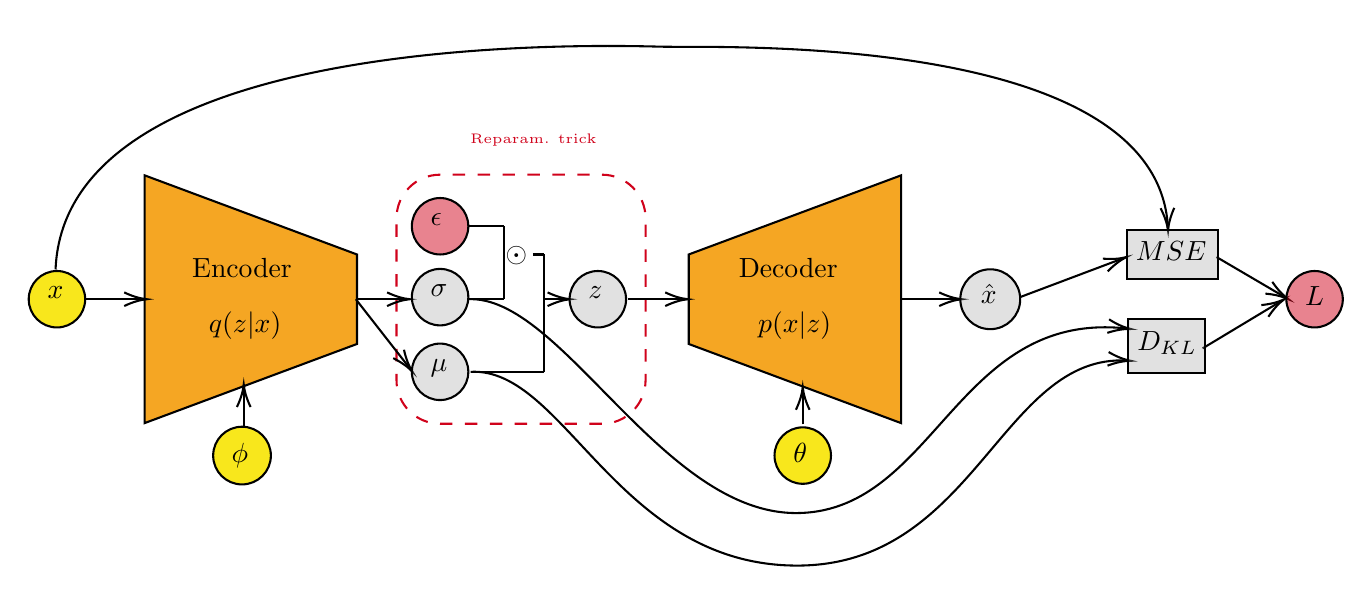
\begin{tikzpicture}[x=0.75pt,y=0.75pt,yscale=-1,xscale=1]
%uncomment if require: \path (0,300); %set diagram left start at 0, and has height of 300

%Shape: Trapezoid [id:dp7823603828525814] 
\draw  [fill={rgb, 255:red, 245; green, 166; blue, 35 }  ,fill opacity=1 ] (93.26,100.32) -- (195.56,138.44) -- (195.56,181.56) -- (93.26,219.68) -- cycle ;
%Flowchart: Alternative Process [id:dp7916519671015572] 
\draw  [color={rgb, 255:red, 208; green, 2; blue, 27 }  ,draw opacity=1 ][dash pattern={on 4.5pt off 4.5pt}] (313.6,100) .. controls (325.2,100) and (334.6,109.4) .. (334.6,121) -- (334.6,199) .. controls (334.6,210.6) and (325.2,220) .. (313.6,220) -- (235.6,220) .. controls (224,220) and (214.6,210.6) .. (214.6,199) -- (214.6,121) .. controls (214.6,109.4) and (224,100) .. (235.6,100) -- cycle ;
%Shape: Trapezoid [id:dp7878502215303758] 
\draw  [fill={rgb, 255:red, 245; green, 166; blue, 35 }  ,fill opacity=1 ] (457.69,219.68) -- (355.39,181.56) -- (355.39,138.44) -- (457.69,100.32) -- cycle ;
%Straight Lines [id:da7022493612643106] 
\draw    (65,160) -- (92.33,160) ;
\draw [shift={(94.33,160)}, rotate = 180] [color={rgb, 255:red, 0; green, 0; blue, 0 }  ][line width=0.75]    (10.93,-3.29) .. controls (6.95,-1.4) and (3.31,-0.3) .. (0,0) .. controls (3.31,0.3) and (6.95,1.4) .. (10.93,3.29)   ;
%Straight Lines [id:da842524726150703] 
\draw    (141,221.67) -- (141,203) ;
\draw [shift={(141,201)}, rotate = 90] [color={rgb, 255:red, 0; green, 0; blue, 0 }  ][line width=0.75]    (10.93,-3.29) .. controls (6.95,-1.4) and (3.31,-0.3) .. (0,0) .. controls (3.31,0.3) and (6.95,1.4) .. (10.93,3.29)   ;
%Straight Lines [id:da6004403121374124] 
\draw    (457.67,160) -- (485,160) ;
\draw [shift={(487,160)}, rotate = 180] [color={rgb, 255:red, 0; green, 0; blue, 0 }  ][line width=0.75]    (10.93,-3.29) .. controls (6.95,-1.4) and (3.31,-0.3) .. (0,0) .. controls (3.31,0.3) and (6.95,1.4) .. (10.93,3.29)   ;
%Straight Lines [id:da6888855782255758] 
\draw    (410.33,220.33) -- (410.33,204.33) ;
\draw [shift={(410.33,202.33)}, rotate = 90] [color={rgb, 255:red, 0; green, 0; blue, 0 }  ][line width=0.75]    (10.93,-3.29) .. controls (6.95,-1.4) and (3.31,-0.3) .. (0,0) .. controls (3.31,0.3) and (6.95,1.4) .. (10.93,3.29)   ;
%Straight Lines [id:da5580691014824746] 
\draw    (249.67,124.84) -- (266.6,124.84) ;
%Straight Lines [id:da0719604636131792] 
\draw    (249,160) -- (266.6,160) ;
%Straight Lines [id:da12715359384818892] 
\draw    (266.6,124.84) -- (266.6,160) ;
%Straight Lines [id:da1128909560545941] 
\draw    (285.67,194.98) -- (250.33,194.98) ;
%Straight Lines [id:da6821248002376252] 
\draw    (285.67,138.44) -- (285.67,194.98) ;
%Straight Lines [id:da18808034763917325] 
\draw    (280.33,138.44) -- (285.67,138.44) ;
%Straight Lines [id:da9818051915598998] 
\draw    (285.67,160) -- (296.33,160) ;
\draw [shift={(298.33,160)}, rotate = 180] [color={rgb, 255:red, 0; green, 0; blue, 0 }  ][line width=0.75]    (10.93,-3.29) .. controls (6.95,-1.4) and (3.31,-0.3) .. (0,0) .. controls (3.31,0.3) and (6.95,1.4) .. (10.93,3.29)   ;
%Straight Lines [id:da15034327030618333] 
\draw    (326.33,160) -- (353,160) ;
\draw [shift={(355,160)}, rotate = 180] [color={rgb, 255:red, 0; green, 0; blue, 0 }  ][line width=0.75]    (10.93,-3.29) .. controls (6.95,-1.4) and (3.31,-0.3) .. (0,0) .. controls (3.31,0.3) and (6.95,1.4) .. (10.93,3.29)   ;
%Straight Lines [id:da5118381101450515] 
\draw    (195,160) -- (219,160) ;
\draw [shift={(221,160)}, rotate = 180] [color={rgb, 255:red, 0; green, 0; blue, 0 }  ][line width=0.75]    (10.93,-3.29) .. controls (6.95,-1.4) and (3.31,-0.3) .. (0,0) .. controls (3.31,0.3) and (6.95,1.4) .. (10.93,3.29)   ;
%Straight Lines [id:da0008605514980692952] 
\draw    (195,160) -- (221.1,193.4) ;
\draw [shift={(222.33,194.98)}, rotate = 232] [color={rgb, 255:red, 0; green, 0; blue, 0 }  ][line width=0.75]    (10.93,-3.29) .. controls (6.95,-1.4) and (3.31,-0.3) .. (0,0) .. controls (3.31,0.3) and (6.95,1.4) .. (10.93,3.29)   ;
%Curve Lines [id:da606983672133339] 
\draw    (249,160) .. controls (294.33,157.67) and (343,265) .. (409,263) .. controls (474.67,261.01) and (484.9,164.64) .. (567.09,174.18) ;
\draw [shift={(568.33,174.33)}, rotate = 187.29] [color={rgb, 255:red, 0; green, 0; blue, 0 }  ][line width=0.75]    (10.93,-3.29) .. controls (6.95,-1.4) and (3.31,-0.3) .. (0,0) .. controls (3.31,0.3) and (6.95,1.4) .. (10.93,3.29)   ;
%Curve Lines [id:da10450467264141716] 
\draw    (250.33,194.98) .. controls (295.67,192.65) and (321,288.33) .. (407.67,288.33) .. controls (493.47,288.33) and (506.09,186.4) .. (566.49,189.54) ;
\draw [shift={(568.33,189.67)}, rotate = 184.92] [color={rgb, 255:red, 0; green, 0; blue, 0 }  ][line width=0.75]    (10.93,-3.29) .. controls (6.95,-1.4) and (3.31,-0.3) .. (0,0) .. controls (3.31,0.3) and (6.95,1.4) .. (10.93,3.29)   ;
%Curve Lines [id:da10659071061601377] 
\draw    (50.33,145.67) .. controls (55,29.67) and (314.33,37.67) .. (342.33,38.33) .. controls (370.19,39) and (581.54,31.08) .. (586.28,125.57) ;
\draw [shift={(586.33,127)}, rotate = 268.41] [color={rgb, 255:red, 0; green, 0; blue, 0 }  ][line width=0.75]    (10.93,-3.29) .. controls (6.95,-1.4) and (3.31,-0.3) .. (0,0) .. controls (3.31,0.3) and (6.95,1.4) .. (10.93,3.29)   ;
%Straight Lines [id:da6109248809176173] 
\draw    (515,159) -- (564.46,140.37) ;
\draw [shift={(566.33,139.67)}, rotate = 159.36] [color={rgb, 255:red, 0; green, 0; blue, 0 }  ][line width=0.75]    (10.93,-3.29) .. controls (6.95,-1.4) and (3.31,-0.3) .. (0,0) .. controls (3.31,0.3) and (6.95,1.4) .. (10.93,3.29)   ;
%Straight Lines [id:da2945225342159614] 
\draw    (609.67,139.67) -- (642.61,158.99) ;
\draw [shift={(644.33,160)}, rotate = 210.39] [color={rgb, 255:red, 0; green, 0; blue, 0 }  ][line width=0.75]    (10.93,-3.29) .. controls (6.95,-1.4) and (3.31,-0.3) .. (0,0) .. controls (3.31,0.3) and (6.95,1.4) .. (10.93,3.29)   ;
%Straight Lines [id:da8512352195616399] 
\draw    (603,183.67) -- (640.62,161.03) ;
\draw [shift={(642.33,160)}, rotate = 148.96] [color={rgb, 255:red, 0; green, 0; blue, 0 }  ][line width=0.75]    (10.93,-3.29) .. controls (6.95,-1.4) and (3.31,-0.3) .. (0,0) .. controls (3.31,0.3) and (6.95,1.4) .. (10.93,3.29)   ;

% Text Node
\draw  [fill={rgb, 255:red, 248; green, 231; blue, 28 }  ,fill opacity=1 ]  (51, 160) circle [x radius= 13.6, y radius= 13.6]   ;
\draw (45,152.4) node [anchor=north west][inner sep=0.75pt]    {$x$};
% Text Node
\draw (114.67,139) node [anchor=north west][inner sep=0.75pt]   [align=left] {Encoder};
% Text Node
\draw (122.67,164.4) node [anchor=north west][inner sep=0.75pt]    {$q( z|x)$};
% Text Node
\draw (378,139) node [anchor=north west][inner sep=0.75pt]   [align=left] {Decoder};
% Text Node
\draw (387.33,164.4) node [anchor=north west][inner sep=0.75pt]    {$p( x|z)$};
% Text Node
\draw  [fill={rgb, 255:red, 155; green, 155; blue, 155 }  ,fill opacity=0.3 ]  (500.67, 160) circle [x radius= 14.42, y radius= 14.42]   ;
\draw (494.67,151.4) node [anchor=north west][inner sep=0.75pt]    {$\hat{x}$};
% Text Node
\draw  [fill={rgb, 255:red, 248; green, 231; blue, 28 }  ,fill opacity=1 ]  (140.17, 235.33) circle [x radius= 13.9, y radius= 13.9]   ;
\draw (133.67,227.73) node [anchor=north west][inner sep=0.75pt]    {$\phi $};
% Text Node
\draw  [fill={rgb, 255:red, 208; green, 2; blue, 27 }  ,fill opacity=0.49 ]  (235.6, 124.84) circle [x radius= 13.6, y radius= 13.6]   ;
\draw (229.6,117.24) node [anchor=north west][inner sep=0.75pt]    {$\epsilon $};
% Text Node
\draw  [fill={rgb, 255:red, 248; green, 231; blue, 28 }  ,fill opacity=1 ]  (410.33, 235.33) circle [x radius= 13.6, y radius= 13.6]   ;
\draw (404.33,227.73) node [anchor=north west][inner sep=0.75pt]    {$\theta $};
% Text Node
\draw  [fill={rgb, 255:red, 155; green, 155; blue, 155 }  ,fill opacity=0.3 ]  (235.6, 159) circle [x radius= 13.6, y radius= 13.6]   ;
\draw (229.6,151.4) node [anchor=north west][inner sep=0.75pt]    {$\sigma $};
% Text Node
\draw  [fill={rgb, 255:red, 155; green, 155; blue, 155 }  ,fill opacity=0.3 ]  (235.6, 194.98) circle [x radius= 13.6, y radius= 13.6]   ;
\draw (229.6,187.38) node [anchor=north west][inner sep=0.75pt]    {$\mu $};
% Text Node
\draw  [fill={rgb, 255:red, 155; green, 155; blue, 155 }  ,fill opacity=0.3 ]  (311.6, 160) circle [x radius= 13.6, y radius= 13.6]   ;
\draw (305.6,152.4) node [anchor=north west][inner sep=0.75pt]    {$z$};
% Text Node
\draw (265.67,132.84) node [anchor=north west][inner sep=0.75pt]    {$\odot $};
% Text Node
\draw  [fill={rgb, 255:red, 155; green, 155; blue, 155 }  ,fill opacity=0.3 ]  (566.33,126.44) -- (610.33,126.44) -- (610.33,150.44) -- (566.33,150.44) -- cycle  ;
\draw (569.33,130.84) node [anchor=north west][inner sep=0.75pt]    {$MSE$};
% Text Node
\draw  [fill={rgb, 255:red, 155; green, 155; blue, 155 }  ,fill opacity=0.3 ]  (567,169.56) -- (604,169.56) -- (604,195.56) -- (567,195.56) -- cycle  ;
\draw (570,173.96) node [anchor=north west][inner sep=0.75pt]    {$D_{KL}$};
% Text Node
\draw (248.67,79) node [anchor=north west][inner sep=0.75pt]  [color={rgb, 255:red, 208; green, 2; blue, 27 }  ,opacity=1 ] [align=left] {{\tiny Reparam. trick}};
% Text Node
\draw  [fill={rgb, 255:red, 208; green, 2; blue, 27 }  ,fill opacity=0.49 ]  (656.93, 160) circle [x radius= 13.6, y radius= 13.6]   ;
\draw (650.93,152.4) node [anchor=north west][inner sep=0.75pt]    {$L$};


\end{tikzpicture}
    \caption[Architecture of Gaussian VAEs.]%
    { Architecture of Gaussian VAEs. The input $x$ is passed through the encoder with parameters $\phi$ producing the mean $\mu$ and the standard deviation $\sigma$ of the Gaussian distribution. The random variable $\epsilon$ is sampled from a standard Gaussian distribution and is used to sample $ z = \mu + \sigma \odot \epsilon$. The sampled $z$ is then passed through the decoder with parameters $\theta$ producing the output $\hat{x}$. The loss function to be minimized is the sum of the MSE reconstruction loss and the KL divergence regularization loss. 
    }
  	\medskip 
	\hspace*{15pt}\hbox{\scriptsize Credit: Adapted from Kingma and Welling~\cite{Kingma_2019} }\label{VAEFigure}
\end{figure}

\section{Vector Quantized VAEs}\label{background:vqvae}

Vector Quantized VAEs (VQ-VAEs) are a variant of VAEs that were introduced in 2017 by Aäron van den Oord et al.~\cite{vqvae}. The VQ-VAEs have shown various improvements over the standard VAEs, such as higher quality of the generated samples, better disentanglement of the latent space, and better generalization to unseen data. ~\cite{vqvae}.

VQ-VAEs have found extensive application across various domains, showcasing their versatility and effectiveness. One very notable application is in the realm of image generation, where models like DALL-E have leveraged the notion of a discrete latent space introduced by VQ-VAEs to generate high-quality and diverse images from textual descriptions~\cite{dalle}. DALL-E, introduced by OpenAI, utilizes VQ-VAEs to map textual input to discrete latent codes, which are then decoded into coherent images that align with the given descriptions. This capability enables the generation of novel and high-quality images based on textual prompts, demonstrating the power of VQ-VAEs in creative AI applications.

Additionally, VQ-VAEs have been applied in speech synthesis, music generation, and text-to-image synthesis tasks, further highlighting their broad utility and effectiveness in various creative and generative tasks~\cite{vqvae2,vqvaespeechsynthesis, musicvqvae,dalle}.

The VQVAEs fundamentally differ in two key ways from VAEs. Firstly, the latent representation is discrete instead of continuous. Secondly, the prior distribution is learned rather than being fixed. The posterior and prior distributions are categorical and the samples taken from these distributions are the indices of the embeddings in the embedding space. These matched indices are then used to look up the embeddings in the embedding space and then used as input to the decoder~\cite{vqvae}. VQ-VAE learning process consists of two stages. In the first stage, the encoder and the decoder are trained. In the second stage a prior over these discrete latent variables is trained~\cite{vqvae}.

\subsection{Discrete Latent Variables}

VQ-VAEs focus on discrete latent variables, which is a more natural fit for many types of data. Language and speech naturally is a stream of discrete units, such as words or phonemes. Images can be often well described by language, which can the discrete representations well-suited for images as well. Moreover, discrete representations work very well with complex reasoning, and decision-making~\cite{vqvae}.

VQ-VAEs define a latent embedding space $ e \in \mathbb{R}^{K \times D} $, where $K$ is the number of embeddings and $D$ is the dimension of each latent embedding vector. The model takes an input $x$, which is passed through the encoder producing output $z_e(x)$, as shown in figure~\ref{VQVAEFigure}. 
The discrete latent variables $z$ are then calculated by nearest neighbor lookup in the embedding space
 \[ z = \argmin_{k} || z_e(x) - e_k ||^2,\] 
where $e_k$ is the $k$-th embedding vector in the embedding space. The decoder then takes the discrete latent variables $z$ and produces the output $\hat{x}$. 
One can see this forward propagation as a regular autoencoder with a quantization step in the middle~\cite{vqvae}.

The posterior categorical distribution $q_{\phi}(z|x)$ is defined as follows:
\begin{equation} \label{eqVQVAEPosterior}
    q(z=k|x) = \begin{cases}
        1& \text{if} \ k = \argmin_{k} || z_e(x) - e_k ||^2 \\
        0& \text{otherwise}
    \end{cases},
\end{equation}
where $z_e(x)$ is the output of the encoder network and $e_k$ is the $k$-th vector in the embedding table.
The discrete latent variable $z$ is then used to look up the corresponding embedding vector $e_k$ in the embedding space, which is then used as input to the decoder network. The decoder network then produces the output $\hat{x}$~\cite{vqvae}.
The decoder distribution $p_{\theta}(x|z)$ is assumed to be a Gaussian distribution.

\subsection{Learning}

As mentioned earlier, the VQ-VAEs introduce learning the prior distribution separately from the posterior distribution. The prior distribution is defined as a categorical distribution $p_{\omega}(z)$, where $z$ is a discrete latent variable~\cite{vqvae}.

Since the proposed posterior distribution $q_{\phi}(z|x)$ is deterministic by applying it to the ELBO objective, we get the following expression:
\begin{equation}
    \begin{split}
        L_{\theta, \phi, \omega}(x) &= - D_{KL}(q_{\phi}(z = k|x) || p_{\omega}(z)) + \mathbb{E}_{q_{\phi}(z=k|x)} [\log p_{\theta}(x|z = k)],\\
                            &= - \mathbb{E}_{q_{\phi}(z=k|x)} [\log \frac{q_{\phi}(z=k|x)}{p_{\omega}(z)}] + \mathbb{E}_{q_{\phi}(z=k|x)} [\log p_{\theta}(x|z = k)],\\
                            &= - \log \frac{1}{p_{\omega}(z)} + \log p_{\theta}(x|z = k),\\
                            &= \log p_{\omega}(z) + \log p_{\theta}(x|z = k),\\
    \end{split}
\end{equation}

The VQVAE learning process is then divided into two stages, where in the first stage the first term is ignored, and the second term is maximized. In the second stage, the prior distribution is trained. In the next 2 sections, I will describe both stages in more detail.

\subsubsection{First stage}

In the first stage, the log-likelihood of the posterior distribution is \textbf{maximized}, which means the encoder and the decoder are trained with the prior distribution being arbitrary. The training objective in the first stages was reduced to 
\[ L_{\theta, \phi}(x) = \log p_{\theta}(x|z = k), \]
where $k$ is the index of the nearest embedding vector in the embedding space, which is defined in equation~\ref{eqVQVAEPosterior}. We can look at the first stage as training a regular autoencoder with a quantization step in the middle, which inherently makes the latent space distribution categorical~\cite{vqvae}.
    
However, the expression $k = \argmin_{k} || z_e(x) - e_k ||^2$ is not differentiable with respect to the parameters of the network. To make the training process differentiable, the authors of the VQ-VAEs propose to use the straight-through estimator, which is a way of estimating the gradients of the non-differentiable function, and copy the gradients of $z_q(x)$ to $z_e(x)$~\cite{vqvae}. The straight-through estimator only works if the difference between $z_e(x)$ and $e_k$ is small, which can be achieved by adding extra loss terms to the training objective.~\cite{straight_through}

This is where the VQ objective comes in. The VQ objective uses the second term of equation~\ref{eqVQVAEObjective} to encourage the encoder to produce representations that are close to the embedding vectors in the embedding space, which is called the commitment loss~\cite{vqvae}.

However, since the embedding space can be arbitrarily large the embedding vectors can be arbitrarily far from the encoder output. To prevent this, the authors of the VQ-VAEs propose to add another term to the training objective, which is called codebook loss. The codebook loss encourages the embedding vectors to be close to the encoder output. The codebook loss has $\beta$ as a hyperparameter, which controls the importance of the codebook loss~\cite{vqvae}.

Thus, the resulting training objective becomes
\begin{equation} \label{eqVQVAEObjective}
    \begin{split}
        L &= \log p_{\theta}(x|z = k) - \biggl( || sg(z_e(x)) - e_k ||^2 + \beta || z_q(x) - sg(e_k) ||^2 \biggr),\\
    \end{split}
\end{equation}
where $sg$ is the stop gradient operation, which is defined as an identity function, but with the gradients of the output set to zero.

The loss function to be \textbf{minimized} for VQ-VAEs usually used in practice is the sum of the VQ objective and the MSE reconstruction loss.
The first term in the function is the MSE reconstruction loss because maximizing the Gaussian likelihood is approximately equivalent to minimizing the MSE reconstruction loss. This is shown in the equation~\ref{eqMSE}. 
Thus, the resulting training objective to be minimized becomes
\[ L = \frac{1}{D} \sum_{i=1}^{D} ||x_i - \hat{x}_i ||^2 + \frac{1}{Z} \sum_{i=1}^{Z} \biggl( || sg(z_e(x))_i - e_{k_{i}} ||^2 + \beta || z_q(x)_i -  sg(e_{k{i}}) ||^2 \biggr), \]
where $\hat{x} = f_{\theta}(z_q(x))$, where function $f_{\theta}$ is the decoder network, $D$ is the dimension of the input data, $Z$ is the number of latent space vectors and $k_{i}$ is the index of the nearest embedding vector in the embedding space for the $i$-th latent space vector, which is defined in equation~\ref{eqVQVAEPosterior}~\cite{vqvae}.

In the figure below~\ref{VQVAEFigure} there is a visualization of the architecture of VQ-VAEs.

\begin{figure}
    \centering 
    

\tikzset{every picture/.style={line width=0.75pt}} %set default line width to 0.75pt        

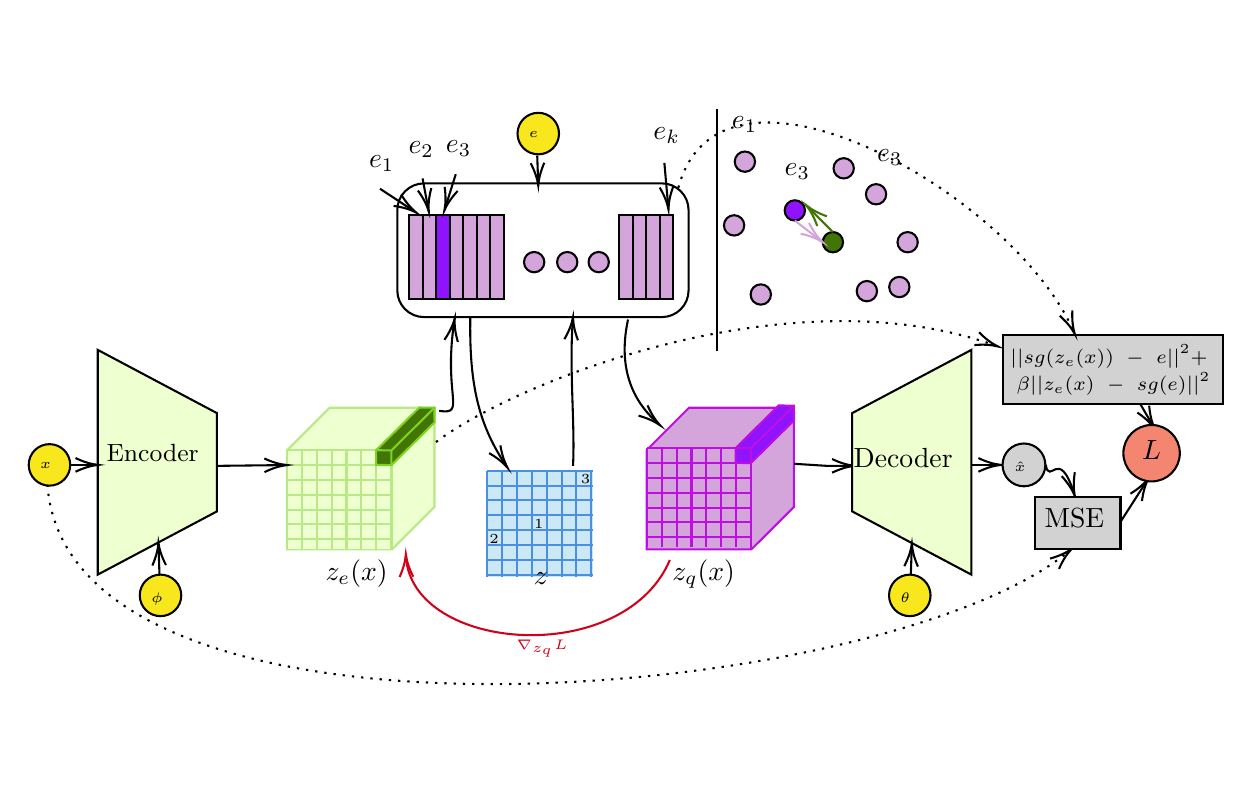
\begin{tikzpicture}[x=0.75pt,y=0.75pt,yscale=-1,xscale=1]
%uncomment if require: \path (0,308); %set diagram left start at 0, and has height of 308

%Shape: Trapezoid [id:dp36465646521888906] 
\draw  [fill={rgb, 255:red, 238; green, 255; blue, 208 }  ,fill opacity=1 ] (97.75,141.72) -- (155.17,172.18) -- (155.17,219.54) -- (97.75,250) -- cycle ;
%Shape: Cube [id:dp9839436955233336] 
\draw  [color={rgb, 255:red, 184; green, 233; blue, 134 }  ,draw opacity=1 ][fill={rgb, 255:red, 238; green, 255; blue, 208 }  ,fill opacity=1 ] (189,190.06) -- (209.47,169.59) -- (260,169.59) -- (260,217.36) -- (239.53,237.83) -- (189,237.83) -- cycle ; \draw  [color={rgb, 255:red, 184; green, 233; blue, 134 }  ,draw opacity=1 ] (260,169.59) -- (239.53,190.06) -- (189,190.06) ; \draw  [color={rgb, 255:red, 184; green, 233; blue, 134 }  ,draw opacity=1 ] (239.53,190.06) -- (239.53,237.83) ;
%Shape: Grid [id:dp5232564483036259] 
\draw  [draw opacity=0][fill={rgb, 255:red, 238; green, 255; blue, 208 }  ,fill opacity=1 ][line width=0.75]  (189,190.06) -- (239.36,190.06) -- (239.36,237.83) -- (189,237.83) -- cycle ; \draw  [color={rgb, 255:red, 184; green, 233; blue, 134 }  ,draw opacity=1 ][line width=0.75]  (189,190.06) -- (189,237.83)(196.15,190.06) -- (196.15,237.83)(203.3,190.06) -- (203.3,237.83)(210.45,190.06) -- (210.45,237.83)(217.6,190.06) -- (217.6,237.83)(224.75,190.06) -- (224.75,237.83)(231.9,190.06) -- (231.9,237.83)(239.05,190.06) -- (239.05,237.83) ; \draw  [color={rgb, 255:red, 184; green, 233; blue, 134 }  ,draw opacity=1 ][line width=0.75]  (189,190.06) -- (239.36,190.06)(189,197.21) -- (239.36,197.21)(189,204.36) -- (239.36,204.36)(189,211.51) -- (239.36,211.51)(189,218.66) -- (239.36,218.66)(189,225.81) -- (239.36,225.81)(189,232.96) -- (239.36,232.96) ; \draw  [color={rgb, 255:red, 184; green, 233; blue, 134 }  ,draw opacity=1 ][line width=0.75]   ;
%Shape: Cube [id:dp6386923890289404] 
\draw  [color={rgb, 255:red, 126; green, 211; blue, 33 }  ,draw opacity=1 ][fill={rgb, 255:red, 65; green, 117; blue, 5 }  ,fill opacity=1 ] (231.89,190.05) -- (252.68,169.48) -- (260,169.59) -- (260.03,176.67) -- (239.25,197.24) -- (231.92,197.13) -- cycle ; \draw  [color={rgb, 255:red, 126; green, 211; blue, 33 }  ,draw opacity=1 ] (260,169.59) -- (239.22,190.16) -- (231.89,190.05) ; \draw  [color={rgb, 255:red, 126; green, 211; blue, 33 }  ,draw opacity=1 ] (239.22,190.16) -- (239.25,197.24) ;
%Shape: Grid [id:dp2868467076547798] 
\draw  [draw opacity=0][fill={rgb, 255:red, 204; green, 232; blue, 244 }  ,fill opacity=1 ][line width=0.75]  (285.5,199.95) -- (336.5,199.95) -- (336.5,250.95) -- (285.5,250.95) -- cycle ; \draw  [color={rgb, 255:red, 74; green, 144; blue, 226 }  ,draw opacity=1 ][line width=0.75]  (285.5,199.95) -- (285.5,250.95)(292.65,199.95) -- (292.65,250.95)(299.8,199.95) -- (299.8,250.95)(306.95,199.95) -- (306.95,250.95)(314.1,199.95) -- (314.1,250.95)(321.25,199.95) -- (321.25,250.95)(328.4,199.95) -- (328.4,250.95)(335.55,199.95) -- (335.55,250.95) ; \draw  [color={rgb, 255:red, 74; green, 144; blue, 226 }  ,draw opacity=1 ][line width=0.75]  (285.5,199.95) -- (336.5,199.95)(285.5,207.1) -- (336.5,207.1)(285.5,214.25) -- (336.5,214.25)(285.5,221.4) -- (336.5,221.4)(285.5,228.55) -- (336.5,228.55)(285.5,235.7) -- (336.5,235.7)(285.5,242.85) -- (336.5,242.85)(285.5,250) -- (336.5,250) ; \draw  [color={rgb, 255:red, 74; green, 144; blue, 226 }  ,draw opacity=1 ][line width=0.75]   ;
%Shape: Cube [id:dp9385697445458008] 
\draw  [color={rgb, 255:red, 189; green, 16; blue, 224 }  ,draw opacity=1 ][fill={rgb, 255:red, 212; green, 165; blue, 219 }  ,fill opacity=1 ] (362.17,190.06) -- (382.64,169.59) -- (433.17,169.59) -- (433.17,217.36) -- (412.69,237.83) -- (362.17,237.83) -- cycle ; \draw  [color={rgb, 255:red, 189; green, 16; blue, 224 }  ,draw opacity=1 ] (433.17,169.59) -- (412.69,190.06) -- (362.17,190.06) ; \draw  [color={rgb, 255:red, 189; green, 16; blue, 224 }  ,draw opacity=1 ] (412.69,190.06) -- (412.69,237.83) ;
%Shape: Grid [id:dp22814793354422447] 
\draw  [draw opacity=0][fill={rgb, 255:red, 212; green, 165; blue, 219 }  ,fill opacity=1 ][line width=0.75]  (362.37,189.11) -- (412.73,189.11) -- (412.73,236.88) -- (362.37,236.88) -- cycle ; \draw  [color={rgb, 255:red, 189; green, 16; blue, 224 }  ,draw opacity=1 ][line width=0.75]  (362.37,189.11) -- (362.37,236.88)(369.52,189.11) -- (369.52,236.88)(376.67,189.11) -- (376.67,236.88)(383.82,189.11) -- (383.82,236.88)(390.97,189.11) -- (390.97,236.88)(398.12,189.11) -- (398.12,236.88)(405.27,189.11) -- (405.27,236.88)(412.42,189.11) -- (412.42,236.88) ; \draw  [color={rgb, 255:red, 189; green, 16; blue, 224 }  ,draw opacity=1 ][line width=0.75]  (362.37,189.11) -- (412.73,189.11)(362.37,196.26) -- (412.73,196.26)(362.37,203.41) -- (412.73,203.41)(362.37,210.56) -- (412.73,210.56)(362.37,217.71) -- (412.73,217.71)(362.37,224.86) -- (412.73,224.86)(362.37,232.01) -- (412.73,232.01) ; \draw  [color={rgb, 255:red, 189; green, 16; blue, 224 }  ,draw opacity=1 ][line width=0.75]   ;
%Rounded Rect [id:dp987340568559665] 
\draw   (242.08,74.38) .. controls (242.08,67.27) and (247.85,61.5) .. (254.97,61.5) -- (369.53,61.5) .. controls (376.65,61.5) and (382.42,67.27) .. (382.42,74.38) -- (382.42,113.03) .. controls (382.42,120.15) and (376.65,125.92) .. (369.53,125.92) -- (254.97,125.92) .. controls (247.85,125.92) and (242.08,120.15) .. (242.08,113.03) -- cycle ;
%Shape: Rectangle [id:dp30823863628595904] 
\draw  [fill={rgb, 255:red, 212; green, 165; blue, 219 }  ,fill opacity=1 ] (247.83,76.83) -- (254.33,76.83) -- (254.33,117) -- (247.83,117) -- cycle ;
%Shape: Rectangle [id:dp5997971655975829] 
\draw  [fill={rgb, 255:red, 212; green, 165; blue, 219 }  ,fill opacity=1 ] (254.33,76.83) -- (260.83,76.83) -- (260.83,117) -- (254.33,117) -- cycle ;
%Shape: Rectangle [id:dp9067829242009235] 
\draw  [fill={rgb, 255:red, 144; green, 19; blue, 254 }  ,fill opacity=1 ] (260.83,76.83) -- (267.33,76.83) -- (267.33,117) -- (260.83,117) -- cycle ;
%Shape: Rectangle [id:dp9839671090206037] 
\draw  [fill={rgb, 255:red, 212; green, 165; blue, 219 }  ,fill opacity=1 ] (267.33,76.83) -- (273.83,76.83) -- (273.83,117) -- (267.33,117) -- cycle ;
%Shape: Rectangle [id:dp637271918983642] 
\draw  [fill={rgb, 255:red, 212; green, 165; blue, 219 }  ,fill opacity=1 ] (273.83,76.83) -- (280.33,76.83) -- (280.33,117) -- (273.83,117) -- cycle ;
%Shape: Rectangle [id:dp6037901670914401] 
\draw  [fill={rgb, 255:red, 212; green, 165; blue, 219 }  ,fill opacity=1 ] (280.33,76.83) -- (286.83,76.83) -- (286.83,117) -- (280.33,117) -- cycle ;
%Shape: Rectangle [id:dp5095550610243931] 
\draw  [fill={rgb, 255:red, 212; green, 165; blue, 219 }  ,fill opacity=1 ] (286.83,76.83) -- (293.33,76.83) -- (293.33,117) -- (286.83,117) -- cycle ;
%Shape: Rectangle [id:dp567247771177326] 
\draw  [fill={rgb, 255:red, 212; green, 165; blue, 219 }  ,fill opacity=1 ] (349,76.83) -- (355.5,76.83) -- (355.5,117) -- (349,117) -- cycle ;
%Shape: Rectangle [id:dp845410248827495] 
\draw  [fill={rgb, 255:red, 212; green, 165; blue, 219 }  ,fill opacity=1 ] (355.5,76.83) -- (362,76.83) -- (362,117) -- (355.5,117) -- cycle ;
%Shape: Rectangle [id:dp6861462857716385] 
\draw  [fill={rgb, 255:red, 212; green, 165; blue, 219 }  ,fill opacity=1 ] (362,76.83) -- (368.5,76.83) -- (368.5,117) -- (362,117) -- cycle ;
%Shape: Rectangle [id:dp4814994913911068] 
\draw  [fill={rgb, 255:red, 212; green, 165; blue, 219 }  ,fill opacity=1 ] (368.5,76.83) -- (375,76.83) -- (375,117) -- (368.5,117) -- cycle ;
%Shape: Circle [id:dp522837592365686] 
\draw  [fill={rgb, 255:red, 212; green, 165; blue, 219 }  ,fill opacity=1 ] (319.06,99.44) .. controls (319.06,96.73) and (321.25,94.54) .. (323.96,94.54) .. controls (326.66,94.54) and (328.85,96.73) .. (328.85,99.44) .. controls (328.85,102.14) and (326.66,104.33) .. (323.96,104.33) .. controls (321.25,104.33) and (319.06,102.14) .. (319.06,99.44) -- cycle ;
%Shape: Circle [id:dp6306767856366036] 
\draw  [fill={rgb, 255:red, 212; green, 165; blue, 219 }  ,fill opacity=1 ] (334.23,99.44) .. controls (334.23,96.73) and (336.42,94.54) .. (339.12,94.54) .. controls (341.83,94.54) and (344.02,96.73) .. (344.02,99.44) .. controls (344.02,102.14) and (341.83,104.33) .. (339.12,104.33) .. controls (336.42,104.33) and (334.23,102.14) .. (334.23,99.44) -- cycle ;
%Shape: Circle [id:dp21003947259846445] 
\draw  [fill={rgb, 255:red, 212; green, 165; blue, 219 }  ,fill opacity=1 ] (303.12,99.44) .. controls (303.12,96.73) and (305.31,94.54) .. (308.02,94.54) .. controls (310.72,94.54) and (312.92,96.73) .. (312.92,99.44) .. controls (312.92,102.14) and (310.72,104.33) .. (308.02,104.33) .. controls (305.31,104.33) and (303.12,102.14) .. (303.12,99.44) -- cycle ;
%Straight Lines [id:da4730245477119335] 
\draw    (233.75,64.09) -- (249.58,74.49) ;
\draw [shift={(251.25,75.59)}, rotate = 213.31] [color={rgb, 255:red, 0; green, 0; blue, 0 }  ][line width=0.75]    (10.93,-3.29) .. controls (6.95,-1.4) and (3.31,-0.3) .. (0,0) .. controls (3.31,0.3) and (6.95,1.4) .. (10.93,3.29)   ;
%Straight Lines [id:da7768631230213965] 
\draw    (254.25,59.09) -- (256.88,73.12) ;
\draw [shift={(257.25,75.09)}, rotate = 259.38] [color={rgb, 255:red, 0; green, 0; blue, 0 }  ][line width=0.75]    (10.93,-3.29) .. controls (6.95,-1.4) and (3.31,-0.3) .. (0,0) .. controls (3.31,0.3) and (6.95,1.4) .. (10.93,3.29)   ;
%Straight Lines [id:da9227058463688853] 
\draw    (270.25,57.09) -- (265.35,72.68) ;
\draw [shift={(264.75,74.59)}, rotate = 287.45] [color={rgb, 255:red, 0; green, 0; blue, 0 }  ][line width=0.75]    (10.93,-3.29) .. controls (6.95,-1.4) and (3.31,-0.3) .. (0,0) .. controls (3.31,0.3) and (6.95,1.4) .. (10.93,3.29)   ;
%Straight Lines [id:da5035350182337077] 
\draw    (370.75,51.59) -- (372.57,72.09) ;
\draw [shift={(372.75,74.09)}, rotate = 264.92] [color={rgb, 255:red, 0; green, 0; blue, 0 }  ][line width=0.75]    (10.93,-3.29) .. controls (6.95,-1.4) and (3.31,-0.3) .. (0,0) .. controls (3.31,0.3) and (6.95,1.4) .. (10.93,3.29)   ;
%Shape: Cube [id:dp5455643438926754] 
\draw  [color={rgb, 255:red, 189; green, 16; blue, 224 }  ,draw opacity=1 ][fill={rgb, 255:red, 144; green, 19; blue, 254 }  ,fill opacity=1 ] (405.07,189.06) -- (425.85,168.49) -- (433.18,168.6) -- (433.21,175.69) -- (412.42,196.26) -- (405.1,196.15) -- cycle ; \draw  [color={rgb, 255:red, 189; green, 16; blue, 224 }  ,draw opacity=1 ] (433.18,168.6) -- (412.39,189.17) -- (405.07,189.06) ; \draw  [color={rgb, 255:red, 189; green, 16; blue, 224 }  ,draw opacity=1 ] (412.39,189.17) -- (412.42,196.26) ;
%Straight Lines [id:da0934101569879584] 
\draw    (433.25,196.59) -- (449,197.59) -- (460.5,197.59) ;
\draw [shift={(462.5,197.59)}, rotate = 180] [color={rgb, 255:red, 0; green, 0; blue, 0 }  ][line width=0.75]    (10.93,-3.29) .. controls (6.95,-1.4) and (3.31,-0.3) .. (0,0) .. controls (3.31,0.3) and (6.95,1.4) .. (10.93,3.29)   ;
%Straight Lines [id:da9792182129604674] 
\draw    (155.75,197.59) -- (187,197.23) ;
\draw [shift={(189,197.21)}, rotate = 179.35] [color={rgb, 255:red, 0; green, 0; blue, 0 }  ][line width=0.75]    (10.93,-3.29) .. controls (6.95,-1.4) and (3.31,-0.3) .. (0,0) .. controls (3.31,0.3) and (6.95,1.4) .. (10.93,3.29)   ;
%Curve Lines [id:da2262261338808227] 
\draw    (277.25,125.92) .. controls (276.76,156.63) and (280.55,176.57) .. (294.18,197.01) ;
\draw [shift={(295.25,198.59)}, rotate = 235.38] [color={rgb, 255:red, 0; green, 0; blue, 0 }  ][line width=0.75]    (10.93,-3.29) .. controls (6.95,-1.4) and (3.31,-0.3) .. (0,0) .. controls (3.31,0.3) and (6.95,1.4) .. (10.93,3.29)   ;
%Curve Lines [id:da9241998830342757] 
\draw    (262.25,171.09) .. controls (275.55,173.06) and (264.1,164.35) .. (269.49,128.25) ;
\draw [shift={(269.75,126.59)}, rotate = 99.09] [color={rgb, 255:red, 0; green, 0; blue, 0 }  ][line width=0.75]    (10.93,-3.29) .. controls (6.95,-1.4) and (3.31,-0.3) .. (0,0) .. controls (3.31,0.3) and (6.95,1.4) .. (10.93,3.29)   ;
%Curve Lines [id:da3327456466588097] 
\draw    (326.75,197.59) .. controls (327.73,177.11) and (324.9,151.72) .. (326.61,127.76) ;
\draw [shift={(326.75,125.92)}, rotate = 94.67] [color={rgb, 255:red, 0; green, 0; blue, 0 }  ][line width=0.75]    (10.93,-3.29) .. controls (6.95,-1.4) and (3.31,-0.3) .. (0,0) .. controls (3.31,0.3) and (6.95,1.4) .. (10.93,3.29)   ;
%Curve Lines [id:da9765543501242715] 
\draw    (353.25,127.09) .. controls (347.14,155.29) and (359.59,169.79) .. (367.33,176.83) ;
\draw [shift={(368.75,178.09)}, rotate = 220.91] [color={rgb, 255:red, 0; green, 0; blue, 0 }  ][line width=0.75]    (10.93,-3.29) .. controls (6.95,-1.4) and (3.31,-0.3) .. (0,0) .. controls (3.31,0.3) and (6.95,1.4) .. (10.93,3.29)   ;
%Shape: Trapezoid [id:dp8428747340164717] 
\draw  [fill={rgb, 255:red, 238; green, 255; blue, 208 }  ,fill opacity=1 ] (518.67,250) -- (461.25,219.54) -- (461.25,172.18) -- (518.67,141.72) -- cycle ;
%Straight Lines [id:da3079769057377866] 
\draw    (396.25,25.59) -- (396.25,142.09) ;
%Shape: Circle [id:dp9948358303216249] 
\draw  [fill={rgb, 255:red, 144; green, 19; blue, 254 }  ,fill opacity=1 ] (428.72,74.53) .. controls (428.72,71.83) and (430.91,69.63) .. (433.62,69.63) .. controls (436.32,69.63) and (438.52,71.83) .. (438.52,74.53) .. controls (438.52,77.24) and (436.32,79.43) .. (433.62,79.43) .. controls (430.91,79.43) and (428.72,77.24) .. (428.72,74.53) -- cycle ;
%Shape: Circle [id:dp5522117322076687] 
\draw  [fill={rgb, 255:red, 212; green, 165; blue, 219 }  ,fill opacity=1 ] (412.32,115.04) .. controls (412.32,112.33) and (414.51,110.14) .. (417.22,110.14) .. controls (419.92,110.14) and (422.12,112.33) .. (422.12,115.04) .. controls (422.12,117.74) and (419.92,119.93) .. (417.22,119.93) .. controls (414.51,119.93) and (412.32,117.74) .. (412.32,115.04) -- cycle ;
%Shape: Circle [id:dp37361306443013786] 
\draw  [fill={rgb, 255:red, 212; green, 165; blue, 219 }  ,fill opacity=1 ] (463.43,113.42) .. controls (463.43,110.71) and (465.62,108.52) .. (468.32,108.52) .. controls (471.03,108.52) and (473.22,110.71) .. (473.22,113.42) .. controls (473.22,116.12) and (471.03,118.32) .. (468.32,118.32) .. controls (465.62,118.32) and (463.43,116.12) .. (463.43,113.42) -- cycle ;
%Shape: Circle [id:dp891940541408015] 
\draw  [fill={rgb, 255:red, 212; green, 165; blue, 219 }  ,fill opacity=1 ] (399.46,81.73) .. controls (399.46,79.03) and (401.65,76.83) .. (404.36,76.83) .. controls (407.06,76.83) and (409.25,79.03) .. (409.25,81.73) .. controls (409.25,84.44) and (407.06,86.63) .. (404.36,86.63) .. controls (401.65,86.63) and (399.46,84.44) .. (399.46,81.73) -- cycle ;
%Shape: Circle [id:dp2010992949282573] 
\draw  [fill={rgb, 255:red, 65; green, 117; blue, 5 }  ,fill opacity=1 ] (447.06,89.84) .. controls (447.06,87.13) and (449.25,84.94) .. (451.96,84.94) .. controls (454.66,84.94) and (456.85,87.13) .. (456.85,89.84) .. controls (456.85,92.54) and (454.66,94.73) .. (451.96,94.73) .. controls (449.25,94.73) and (447.06,92.54) .. (447.06,89.84) -- cycle ;
%Shape: Circle [id:dp6580309194400682] 
\draw  [fill={rgb, 255:red, 212; green, 165; blue, 219 }  ,fill opacity=1 ] (452.26,54.24) .. controls (452.26,51.53) and (454.45,49.34) .. (457.16,49.34) .. controls (459.86,49.34) and (462.05,51.53) .. (462.05,54.24) .. controls (462.05,56.94) and (459.86,59.13) .. (457.16,59.13) .. controls (454.45,59.13) and (452.26,56.94) .. (452.26,54.24) -- cycle ;
%Shape: Circle [id:dp3786180692063268] 
\draw  [fill={rgb, 255:red, 212; green, 165; blue, 219 }  ,fill opacity=1 ] (467.86,66.74) .. controls (467.86,64.03) and (470.05,61.84) .. (472.76,61.84) .. controls (475.46,61.84) and (477.65,64.03) .. (477.65,66.74) .. controls (477.65,69.44) and (475.46,71.63) .. (472.76,71.63) .. controls (470.05,71.63) and (467.86,69.44) .. (467.86,66.74) -- cycle ;
%Shape: Circle [id:dp5880744034956527] 
\draw  [fill={rgb, 255:red, 212; green, 165; blue, 219 }  ,fill opacity=1 ] (483.06,89.84) .. controls (483.06,87.13) and (485.25,84.94) .. (487.96,84.94) .. controls (490.66,84.94) and (492.85,87.13) .. (492.85,89.84) .. controls (492.85,92.54) and (490.66,94.73) .. (487.96,94.73) .. controls (485.25,94.73) and (483.06,92.54) .. (483.06,89.84) -- cycle ;
%Shape: Circle [id:dp7728747717342119] 
\draw  [fill={rgb, 255:red, 212; green, 165; blue, 219 }  ,fill opacity=1 ] (479.06,111.44) .. controls (479.06,108.73) and (481.25,106.54) .. (483.96,106.54) .. controls (486.66,106.54) and (488.85,108.73) .. (488.85,111.44) .. controls (488.85,114.14) and (486.66,116.33) .. (483.96,116.33) .. controls (481.25,116.33) and (479.06,114.14) .. (479.06,111.44) -- cycle ;
%Shape: Circle [id:dp8092299894843566] 
\draw  [fill={rgb, 255:red, 212; green, 165; blue, 219 }  ,fill opacity=1 ] (404.66,51.04) .. controls (404.66,48.33) and (406.85,46.14) .. (409.56,46.14) .. controls (412.26,46.14) and (414.45,48.33) .. (414.45,51.04) .. controls (414.45,53.74) and (412.26,55.93) .. (409.56,55.93) .. controls (406.85,55.93) and (404.66,53.74) .. (404.66,51.04) -- cycle ;
%Straight Lines [id:da48440557106316784] 
\draw [color={rgb, 255:red, 212; green, 165; blue, 219 }  ,draw opacity=1 ]   (433.62,79.43) -- (445.48,88.61) ;
\draw [shift={(447.06,89.84)}, rotate = 217.76] [color={rgb, 255:red, 212; green, 165; blue, 219 }  ,draw opacity=1 ][line width=0.75]    (10.93,-3.29) .. controls (6.95,-1.4) and (3.31,-0.3) .. (0,0) .. controls (3.31,0.3) and (6.95,1.4) .. (10.93,3.29)   ;
%Straight Lines [id:da1905841532534014] 
\draw [color={rgb, 255:red, 65; green, 117; blue, 5 }  ,draw opacity=1 ][fill={rgb, 255:red, 65; green, 117; blue, 5 }  ,fill opacity=1 ]   (451.96,84.94) -- (440.41,73.35) ;
\draw [shift={(439,71.94)}, rotate = 45.1] [color={rgb, 255:red, 65; green, 117; blue, 5 }  ,draw opacity=1 ][line width=0.75]    (10.93,-3.29) .. controls (6.95,-1.4) and (3.31,-0.3) .. (0,0) .. controls (3.31,0.3) and (6.95,1.4) .. (10.93,3.29)   ;
%Straight Lines [id:da3646207939780566] 
\draw    (84.5,197.13) -- (96,197.13) ;
\draw [shift={(98,197.13)}, rotate = 180] [color={rgb, 255:red, 0; green, 0; blue, 0 }  ][line width=0.75]    (10.93,-3.29) .. controls (6.95,-1.4) and (3.31,-0.3) .. (0,0) .. controls (3.31,0.3) and (6.95,1.4) .. (10.93,3.29)   ;
%Straight Lines [id:da7414471835536174] 
\draw    (127.5,250) -- (127.06,236.59) ;
\draw [shift={(127,234.59)}, rotate = 88.14] [color={rgb, 255:red, 0; green, 0; blue, 0 }  ][line width=0.75]    (10.93,-3.29) .. controls (6.95,-1.4) and (3.31,-0.3) .. (0,0) .. controls (3.31,0.3) and (6.95,1.4) .. (10.93,3.29)   ;
%Straight Lines [id:da6532112868086741] 
\draw    (489.5,250) -- (489.93,237.09) ;
\draw [shift={(490,235.09)}, rotate = 91.92] [color={rgb, 255:red, 0; green, 0; blue, 0 }  ][line width=0.75]    (10.93,-3.29) .. controls (6.95,-1.4) and (3.31,-0.3) .. (0,0) .. controls (3.31,0.3) and (6.95,1.4) .. (10.93,3.29)   ;
%Straight Lines [id:da567944360754334] 
\draw    (309.5,48.09) -- (309.93,60.59) ;
\draw [shift={(310,62.59)}, rotate = 268.03] [color={rgb, 255:red, 0; green, 0; blue, 0 }  ][line width=0.75]    (10.93,-3.29) .. controls (6.95,-1.4) and (3.31,-0.3) .. (0,0) .. controls (3.31,0.3) and (6.95,1.4) .. (10.93,3.29)   ;
%Straight Lines [id:da5426639611340927] 
\draw    (519,197.13) -- (531,197.13) ;
\draw [shift={(533,197.13)}, rotate = 180] [color={rgb, 255:red, 0; green, 0; blue, 0 }  ][line width=0.75]    (10.93,-3.29) .. controls (6.95,-1.4) and (3.31,-0.3) .. (0,0) .. controls (3.31,0.3) and (6.95,1.4) .. (10.93,3.29)   ;
%Curve Lines [id:da3458703024373422] 
\draw  [dash pattern={on 0.84pt off 2.51pt}]  (73.5,206.59) .. controls (83.45,346.89) and (477.53,311.95) .. (565.69,238.7) ;
\draw [shift={(567,237.59)}, rotate = 139.12] [color={rgb, 255:red, 0; green, 0; blue, 0 }  ][line width=0.75]    (10.93,-3.29) .. controls (6.95,-1.4) and (3.31,-0.3) .. (0,0) .. controls (3.31,0.3) and (6.95,1.4) .. (10.93,3.29)   ;
%Curve Lines [id:da6339473919323386] 
\draw  [dash pattern={on 0.84pt off 2.51pt}]  (260.75,186.09) .. controls (300.55,156.24) and (432.17,104.61) .. (530.03,139.56) ;
\draw [shift={(531.5,140.09)}, rotate = 200.17] [color={rgb, 255:red, 0; green, 0; blue, 0 }  ][line width=0.75]    (10.93,-3.29) .. controls (6.95,-1.4) and (3.31,-0.3) .. (0,0) .. controls (3.31,0.3) and (6.95,1.4) .. (10.93,3.29)   ;
%Curve Lines [id:da9053875872036645] 
\draw    (554.5,197.13) .. controls (556.45,207.33) and (560.78,188.1) .. (567.94,210.3) ;
\draw [shift={(568.5,212.09)}, rotate = 253.3] [color={rgb, 255:red, 0; green, 0; blue, 0 }  ][line width=0.75]    (10.93,-3.29) .. controls (6.95,-1.4) and (3.31,-0.3) .. (0,0) .. controls (3.31,0.3) and (6.95,1.4) .. (10.93,3.29)   ;
%Straight Lines [id:da6669066474499481] 
\draw    (590.5,224.59) -- (602.92,205.28) ;
\draw [shift={(604,203.59)}, rotate = 122.74] [color={rgb, 255:red, 0; green, 0; blue, 0 }  ][line width=0.75]    (10.93,-3.29) .. controls (6.95,-1.4) and (3.31,-0.3) .. (0,0) .. controls (3.31,0.3) and (6.95,1.4) .. (10.93,3.29)   ;
%Shape: Rectangle [id:dp9130971852580467] 
\draw  [fill={rgb, 255:red, 210; green, 210; blue, 210 }  ,fill opacity=1 ] (534,134.71) -- (640,134.71) -- (640,167.71) -- (534,167.71) -- cycle ;
%Straight Lines [id:da6493785264569487] 
\draw    (600,167.71) -- (605.99,177.98) ;
\draw [shift={(607,179.71)}, rotate = 239.74] [color={rgb, 255:red, 0; green, 0; blue, 0 }  ][line width=0.75]    (10.93,-3.29) .. controls (6.95,-1.4) and (3.31,-0.3) .. (0,0) .. controls (3.31,0.3) and (6.95,1.4) .. (10.93,3.29)   ;
%Curve Lines [id:da9064943672927692] 
\draw  [dash pattern={on 0.84pt off 2.51pt}]  (377.5,63.59) .. controls (397.9,-13.02) and (539.08,66.29) .. (568.07,133.09) ;
\draw [shift={(568.5,134.09)}, rotate = 247.32] [color={rgb, 255:red, 0; green, 0; blue, 0 }  ][line width=0.75]    (10.93,-3.29) .. controls (6.95,-1.4) and (3.31,-0.3) .. (0,0) .. controls (3.31,0.3) and (6.95,1.4) .. (10.93,3.29)   ;
%Curve Lines [id:da5299666678217625] 
\draw [color={rgb, 255:red, 208; green, 2; blue, 27 }  ,draw opacity=1 ]   (373.4,242.94) .. controls (351.22,295.22) and (249.46,287.51) .. (246.27,241.55) ;
\draw [shift={(246.2,240.14)}, rotate = 88.54] [color={rgb, 255:red, 208; green, 2; blue, 27 }  ,draw opacity=1 ][line width=0.75]    (10.93,-3.29) .. controls (6.95,-1.4) and (3.31,-0.3) .. (0,0) .. controls (3.31,0.3) and (6.95,1.4) .. (10.93,3.29)   ;

% Text Node
\draw (206,241.4) node [anchor=north west][inner sep=0.75pt]    {$z_{e}( x)$};
% Text Node
\draw (373.17,241.4) node [anchor=north west][inner sep=0.75pt]    {$z_{q}( x)$};
% Text Node
\draw (227,46.4) node [anchor=north west][inner sep=0.75pt]    {$e_{1}$};
% Text Node
\draw (246,39.9) node [anchor=north west][inner sep=0.75pt]    {$e_{2}$};
% Text Node
\draw (264,39.4) node [anchor=north west][inner sep=0.75pt]    {$e_{3}$};
% Text Node
\draw (364,32.9) node [anchor=north west][inner sep=0.75pt]    {$e_{k}$};
% Text Node
\draw (329,200.4) node [anchor=north west][inner sep=0.75pt]  [font=\tiny]  {$3$};
% Text Node
\draw (100.5,185.5) node [anchor=north west][inner sep=0.75pt]   [align=left] {{\small Encoder}};
% Text Node
\draw (460.5,187.5) node [anchor=north west][inner sep=0.75pt]   [align=left] {Decoder};
% Text Node
\draw (427.2,50.4) node [anchor=north west][inner sep=0.75pt]   [align=left] {$\displaystyle e_{3}$};
% Text Node
\draw (401.8,27.6) node [anchor=north west][inner sep=0.75pt]    {$e_{1}$};
% Text Node
\draw (471.8,43.6) node [anchor=north west][inner sep=0.75pt]    {$e_{3}$};
% Text Node
\draw  [fill={rgb, 255:red, 248; green, 231; blue, 28 }  ,fill opacity=1 ]  (128, 260) circle [x radius= 10, y radius= 10]   ;
\draw (122,257.4) node [anchor=north west][inner sep=0.75pt]  [font=\tiny]  {$\phi $};
% Text Node
\draw  [fill={rgb, 255:red, 248; green, 231; blue, 28 }  ,fill opacity=1 ]  (489, 260) circle [x radius= 10, y radius= 10]   ;
\draw (483,257.4) node [anchor=north west][inner sep=0.75pt]  [font=\tiny]  {$\theta $};
% Text Node
\draw  [fill={rgb, 255:red, 248; green, 231; blue, 28 }  ,fill opacity=1 ]  (74.5, 197.13) circle [x radius= 10, y radius= 10]   ;
\draw (68.5,194.53) node [anchor=north west][inner sep=0.75pt]  [font=\tiny]  {$x$};
% Text Node
\draw  [fill={rgb, 255:red, 210; green, 210; blue, 210 }  ,fill opacity=1 ]  (544, 197.13) circle [x radius= 10.31, y radius= 10.31]   ;
\draw (538,194.03) node [anchor=north west][inner sep=0.75pt]  [font=\tiny]  {$\hat{x}$};
% Text Node
\draw  [fill={rgb, 255:red, 248; green, 231; blue, 28 }  ,fill opacity=1 ]  (310, 37.5) circle [x radius= 10, y radius= 10]   ;
\draw (304,34.9) node [anchor=north west][inner sep=0.75pt]  [font=\tiny]  {$e$};
% Text Node
\draw  [fill={rgb, 255:red, 210; green, 210; blue, 210 }  ,fill opacity=1 ]  (549.5,212.5) -- (590.5,212.5) -- (590.5,237.5) -- (549.5,237.5) -- cycle  ;
\draw (552.5,216.5) node [anchor=north west][inner sep=0.75pt]   [align=left] {MSE};
% Text Node
\draw  [fill={rgb, 255:red, 244; green, 134; blue, 113 }  ,fill opacity=1 ]  (605.5, 191.5) circle [x radius= 13.6, y radius= 13.6]   ;
\draw (599.5,183.9) node [anchor=north west][inner sep=0.75pt]    {$L$};
% Text Node
\draw (306.5,221.9) node [anchor=north west][inner sep=0.75pt]  [font=\tiny]  {$1$};
% Text Node
\draw (285,229.06) node [anchor=north west][inner sep=0.75pt]  [font=\tiny]  {$2$};
% Text Node
\draw (536,137.71) node [anchor=north west][inner sep=0.75pt]  [font=\scriptsize] [align=left] {$\displaystyle ||sg( z_{e}( x)) \ -\ e||^{2} +$};
% Text Node
\draw (539,151) node [anchor=north west][inner sep=0.75pt]  [font=\scriptsize] [align=left] {$\displaystyle \beta ||z_{e}( x) \ -\ sg( e) ||^{2}$};
% Text Node
\draw (306.4,247.6) node [anchor=north west][inner sep=0.75pt]    {$z$};
% Text Node
\draw (298,279.94) node [anchor=north west][inner sep=0.75pt]  [font=\tiny,color={rgb, 255:red, 208; green, 2; blue, 27 }  ,opacity=1 ]  {$\nabla _{z_{q}} L$};


\end{tikzpicture}

    \caption[Architecture of VQ-VAEs.]%
    { 
        Architecture of VQ-VAEs. The input $x$ is passed through the encoder convolutional neural network producing the output $z_e(x)$. For each output vector in $z_e(x)$, the nearest embedding vector in the embedding table $e$ is found. The indices of the nearest embedding vectors are then used as the discrete latent variables $z$. The discrete latent variables $z$ are then used to look up and retrieve the corresponding embedding vectors. The retrieved embedding vectors are then used as input to the decoder convolutional neural network producing the output $\hat{x}$. During the backward pass the gradients of the gradients of $z_q(x)$ are copied to $z_e(x)$ using the straight-through estimator, which is illustrated with a red arrow.
        Upper Left: The visualization of the embedding space during training.  The encoder output vector is shown as a dark green dot and the nearest embedding vector is shown as a dark purple dot. The commitment and codebook loss encourage both the encoder output vector and the nearest embedding vector to be close to each other~\cite{vqvae}.
    }
  	\medskip 
	\hspace*{15pt}\hbox{\scriptsize Credit: Adapted from Aäron van den Oord et al.~\cite{vqvae}.}\label{VQVAEFigure}
\end{figure}

\subsubsection{Second stage}

The second stage objective is to train the prior distribution $p_{\omega}(z)$ over the discrete latent variables. The latent variables $z$ are sampled from the posterior distribution $q_{\phi}(z|x)$, which is defined in equation~\ref{eqVQVAEPosterior}. The prior distribution is categorical and can be made autoregressive by depending on other latent variables $z$~\cite{vqvae}.

The prior distribution $p_{\omega}(z)$ is then trained to match the distribution of the latent variables $z$ sampled from the posterior distribution $q_{\phi}(z|x)$. To achieve this the authors of the VQ-VAEs use an autoregressive model to model the prior distribution. The autoregressive model authors used is a Gated PixelCNN, which is a variant of PixelCNN, which is described in \autoref{background:pixelcnn}~\cite{vqvae}.

\section{Semi-Conditioned VAEs}

Semi-conditional VAEs were first introduced in 2020~\cite{Gundersen_2021}. Semi-conditional VAEs (SCVAEs) are a variant of VAEs that were first designed for the reconstruction of non-linear dynamic processes based on sparse observations. The semi-conditional VAEs extend the standard VAEs framework by adding an additional input $m$ to the decoder network $p_{\theta}(x|z, m)$, which is used to condition the decoder on the additional information. 

The additional information $m$ can be any type of information that is available at the time of the reconstruction and can be used to improve the reconstruction of the data. In the original paper, the authors used the SCVAEs to reconstruct fluid flow data. The additional information $m$ was the sparse measurements of the flow data. The method was showcased on two different datasets, velocity data from simulations of 2D flow around a cylinder, and bottom currents~\cite{Gundersen_2021}.

Natural applications for the SCVAEs are related to domains where there are often sparse measurements, such as environmental data. However, the SCVAEs can also be used, for instance, in computer vision to generate new images based on sparse pixel representations~\cite{Gundersen_2021}.

The semi-conditional property of the SCVAEs could also be applied to the VQ-VAEs, which has not been explored yet in the literature. Also, the potential of combining non-conditioned and semi-conditioned VAEs through multitask learning has not been explored yet.

\section{Multitask Learning}

Multitask learning is a machine learning paradigm where multiple tasks are learned at the same time, which has the aim of leveraging the shared information between the tasks to improve the performance of the individual tasks. Unlike traditional single-task learning, where each task is learned independently, multitask learning allows taking advantage of task relationships and learning a shared representation that is useful for all tasks~\cite{multitasklearning}.

The notion of using multitask learning comes from the observation that the tasks are often related and depend on the same underlying features. This can be beneficial in scenarios where the data is limited, which is often the case for medical data~\cite{medicalMultiTask}.

For example, in medical image analysis, in a scenario where the task is to develop a system for identifying and classifying different types of abnormalities in medical images. Traditionally this could be done by training a separate model for each type of abnormality. However, this approach is not optimal due to limited data and the shared features that could be used to identify and classify multiple types of abnormalities~\cite{multitasklearning}.

Multitask learning is an approach in which a single model is trained to perform multiple tasks. In the context of medical image analysis, this could involve training multitask VAE or VQVAE models capable of simultaneously learning to reconstruct images, whilst also learning to classify different types of conditions. 

Multitask learning has been shown to be most effective when the tasks are related and data is limited. The potential and flexibility of multitask learning for improving the model performance make it a very valuable technique in machine learning. It has an unexplored potential in the context of VAEs and VQ-VAEs, which is the main motivation for this thesis.

\section{Additional concepts}

\subsection{PixelCNN}\label{background:pixelcnn}

The PixelCNNs are a prominent autoregressive architecture used in the field of pixel-level prediction. These models operate on images at the level of each individual pixel, learning to generate images or predict missing pixels one at a time. Deep autoregressive models have been shown to be very effective at modeling the full distribution and generating relatively low-resolution images. Generating high-resolution images with merely autoregressive models is challenging because the size of the network increases rapidly with the size of the image~\cite{pixelcnn, pixelrnn}.

Autoregressive models treat an image as a sequence of pixels and the goal is to model the conditional distribution of each pixel given the previous pixels.
Image $x$ is represented as a one-dimensional sequence of pixels $x = (x_1, x_2, \dots, x_N)$, where $x_i$ is the $i$-th pixel in the image and $N$ is the number of pixels in the image. The estimate of the joint distribution of the pixels over an image $x$ is given by the product of the conditional distributions of each pixel given the previous pixels
\[ p(x) = \prod_{i=1}^{N} p(x_i|x_1, x_2, \dots, x_{i-1}),\]
where $p(x_i|x_1, x_2, \dots, x_{i-1})$ is the conditional distribution of the $i$-th pixel given the previous pixels. The generational process of the image is then done by sampling each pixel sequentially from the conditional distribution of the pixel given the previous pixels, which is shown in the figure~\ref{PixelCNNFigure}~\cite{pixelcnn}.


\begin{figure}
    \centering 
    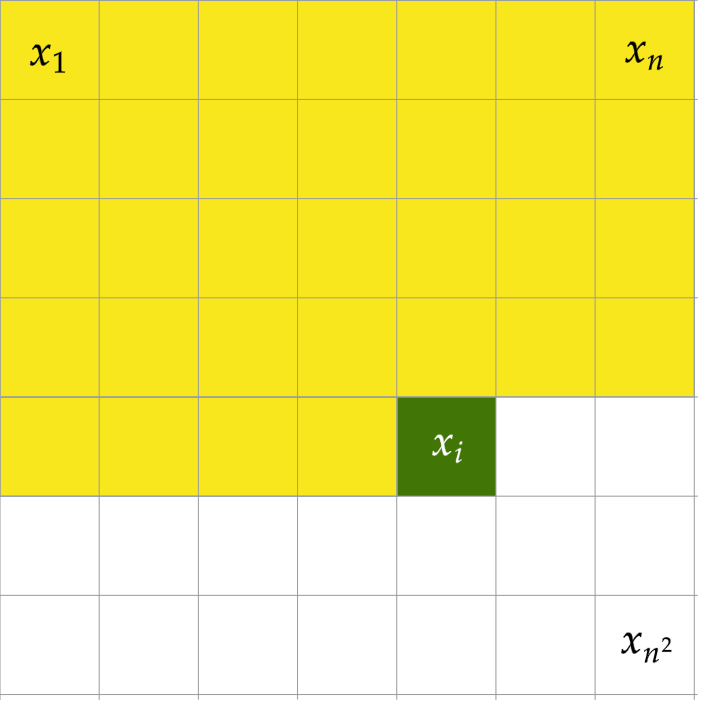
\includegraphics[scale=0.20]{figures/pixelcnn.png}
    \caption[Conditional generation in autoregressive models]%
    {Conditional generation in autoregressive models. The model generates the pixels of the image one at a time, conditioning the previous pixels. The model is autoregressive because the distribution of each pixel is conditioned on the previous pixels.}
  	\medskip 
    \hspace*{15pt}\hbox{\scriptsize Credit: Adapted from the original PixelCNN paper~\cite{pixelcnn}.}\label{PixelCNNFigure}
\end{figure}

The PixelCNN in the original architecture is a stack of fifteen fully convolutional network layers with masked convolutions. The masked convolutions are used to ensure that the model can only access the previous pixels, which is crucial for the model to be autoregressive. The model is trained to minimize the negative log-likelihood of the training data. The PixelCNNs have been shown to be very effective at capturing the distribution of the data. Most current state-of-the-art models use the PixelCNNs as a building block for example PixelCNN++ and PixelSNAIL~\cite{pixelcnn, pixelcnnpp,pixelsnail}.

\subsubsection{Application in VQ-VAEs}

The PixelCNNs are used in the VQ-VAEs to model the prior distribution $p_{\omega}(z)$ over the discrete latent variables. The prior distribution is trained to match the distribution of the latent variables $z$ sampled from the posterior distribution $q_{\phi}(z|x)$. The PixelCNN in combination with the VQ-VAEs has been shown to be exceptional at capturing the distribution of the latent variables and generating high-resolution samples~\cite{vqvae}.


\subsection{Random number generation using Power law distribution}

Power law distribution in probability theory and statistics is a distribution in which one variable is proportional to the power of the other, i.e., 
$p(x) \propto x^{\alpha}$, where $x$ is the random variable and $\alpha$ is the exponent parameter, where $\alpha$ determines the shape of the distribution. The power law distribution is a heavy-tailed distribution, which means that the probability of the large values is higher than in the normal distribution. The power law distribution is used in various fields, such as physics, biology, economics, and computer science~\cite{powerlaw}. 

One example of the power law distribution could be the function $ f(x) = \alpha x^{\alpha - 1} $ for $ 0 \leq x \leq 1 $, $a > 0$. One advantage to this distribution is that this distribution has a finite range and is easy to scale to any range. This fact will be used when power law distribution is used to sample the number of pixels to be conditioned on in the semi-conditional VAEs.

\subsection{SoftAdapt: Adaptive loss weighting} \label{background:softadapt}

SoftAdapt is a novel approach to address the challenge of dynamically adjusting weights for multipart loss functions in deep learning. 
In machine learning, multipart loss functions are common, wherein the loss function is composed of a sum of loss terms. Traditionally, the loss terms of multipart loss function are weighted equally, or their weights are determined through heuristic methods. Whilst this approach can work well in practice, it is not optimal because the importance of the loss terms can vary during the training process and the optimal weights can be hard to determine~\cite{softadapt}.

The approach of the SoftAdapt algorithm which was published in 2020 is to mathematically determine the optimal weights of the loss terms given a short loss history. By evaluating the rate of change for each loss term, it tries to dynamically learn the optimal weights for the loss terms and adapt them during the training process~\cite{softadapt}. The SoftAdapt algorithm since its publication has been shown to be effective in various machine learning applications, such as generative models, model compression and physics-informed neural networks.














